

\begin{figure}[ht]
\begin{minipage}[height=.32\textheight]{.45\textwidth}
\centering \small{\texttt{(a)}}
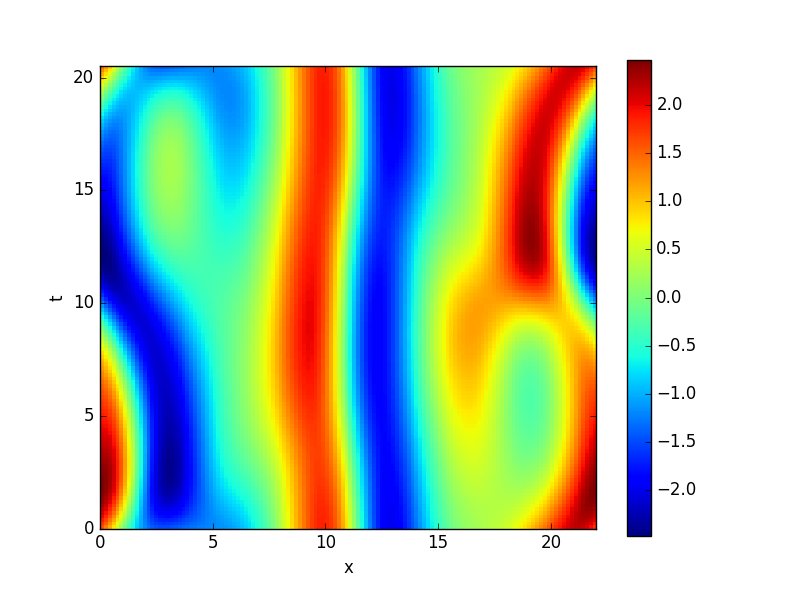
\includegraphics[width=\textwidth,height=.32\textheight]{MNGspacetimeinit1}
\end{minipage}
\begin{minipage}[height=.32\textheight]{.45\textwidth}
\centering \small{\texttt{(b)}}
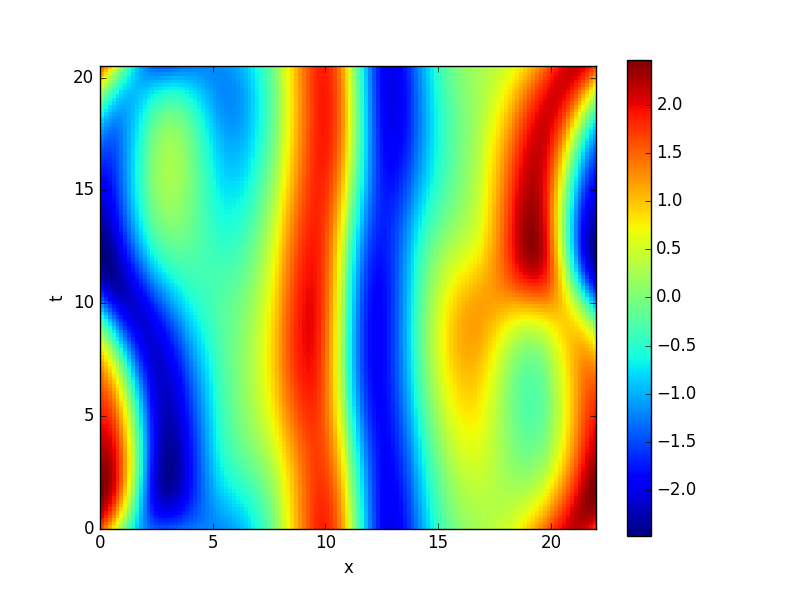
\includegraphics[width=\textwidth,height=.32\textheight]{MNGspacetimefinal1}
\end{minipage}
\caption{ \label{fig:MNGspacetime11}
(a) Initial condition of the 32-by-32 space-by-time discretization of \ppo{10.2}:
$(L_0,\period{0}) = (L_0, 2\period{p_0})= (22,20.5057459345)$.
(b) Resulting spatiotemporal fixed point
$(L_p,2\period{p}) =  (22.0000104401, 20.5057499188)$
}
\end{figure}

\begin{figure}
\begin{minipage}[height=.32\textheight]{.45\textwidth}
\centering \small{\texttt{(a)}}
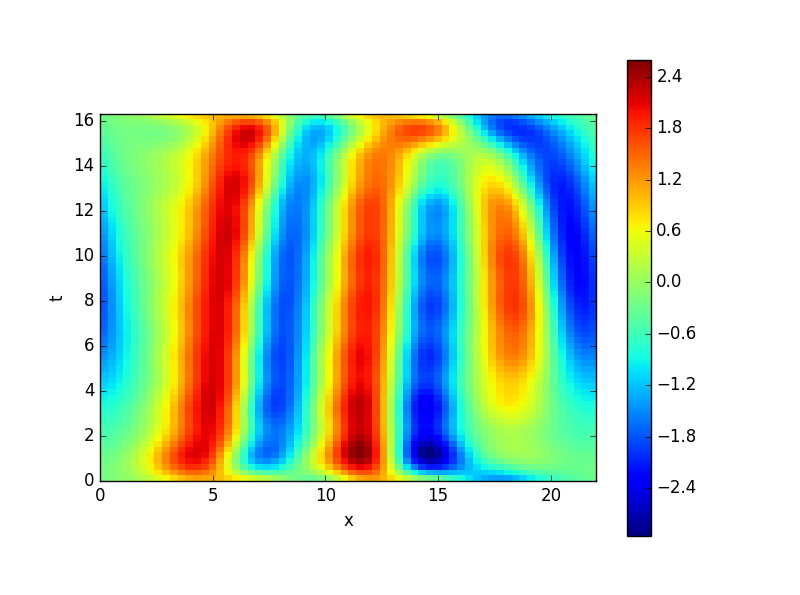
\includegraphics[width=\textwidth,height=.32\textheight]{MNGvndspaceinit2}
\end{minipage}
\\
\begin{minipage}[height=.32\textheight]{.45\textwidth}
\centering \small{\texttt{(b)}}
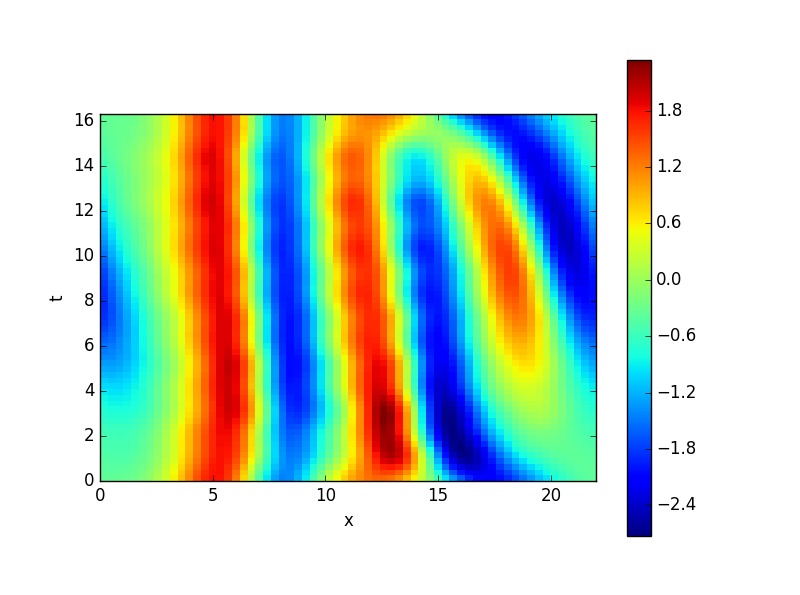
\includegraphics[width=\textwidth,height=.32\textheight]{MNGvndtimefinal2}
\end{minipage}
\begin{minipage}[height=.32\textheight]{.45\textwidth}
\centering \small{\texttt{(c)}}
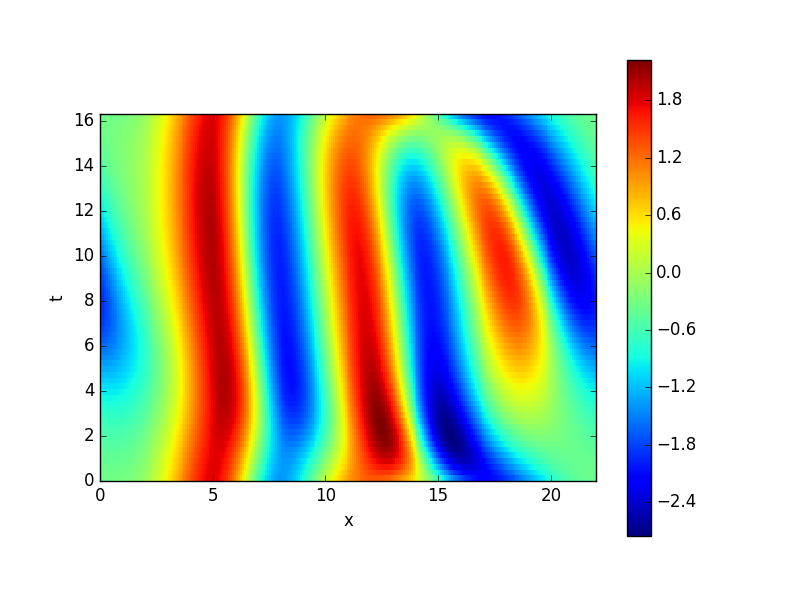
\includegraphics[width=\textwidth,height=.32\textheight]{MNGvndspacefinal2L}
\end{minipage}
\caption{ \label{fig:MNGspaceandtime1}
(a) Initial condition of the 16-by-16 space-by-time discretization of
\rpo{16.31}. $L_0 = 22$.
(b) Resulting periodic orbit after variational {newton descent} in time $L =
22, T = 15.7444884386$,
(c) resulting periodic orbit after variational {newton descent} in space.
%%%lost the number for final spatial size will need to run code again.
}
\end{figure}


\begin{figure}[ht]
\begin{minipage}[height=.32\textheight]{.45\textwidth}
\centering \small{\texttt{(a)}}
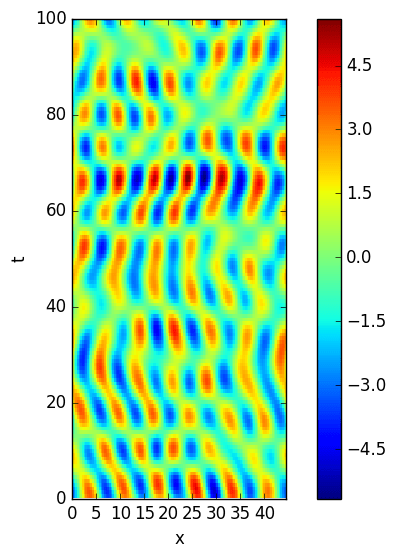
\includegraphics[width=\textwidth,height=.32\textheight]{MNG_T100L44_init}
\end{minipage}
\begin{minipage}[height=.32\textheight]{.45\textwidth}
\centering \small{\texttt{(b)}}
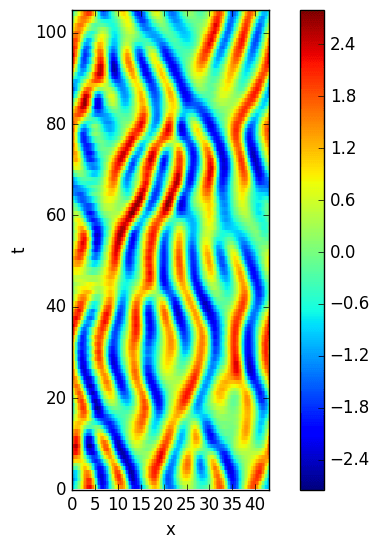
\includegraphics[width=\textwidth,height=.32\textheight]{MNG_T100L44_final}
\end{minipage}
\caption{ \label{fig:MNG_spacetime_smoothed}
(a) Smoothed and $\bar{L}=2\pi\sqrt{2}$ modulated ``noise''
initialized on a spacetime domain
$(L_0,T_0)=(5\bar{L},100)=(44.4,100)$. Initial residual $F^2 = 1808$.
(b) Resultant \twot\ after meeting tolerance
$F(\tau)^2= 1.86<10^{-3} F(0)^2$.
$(L_f,T_f)=(43.066,105.08) = (L_0 - 1.363,T_0 + 5.08)$.
The computation took only 7 CPU seconds on my laptop.
}
\end{figure}

\begin{figure}
\begin{minipage}[height=.32\textheight]{.45\textwidth}
\centering \small{\texttt{(a)}}
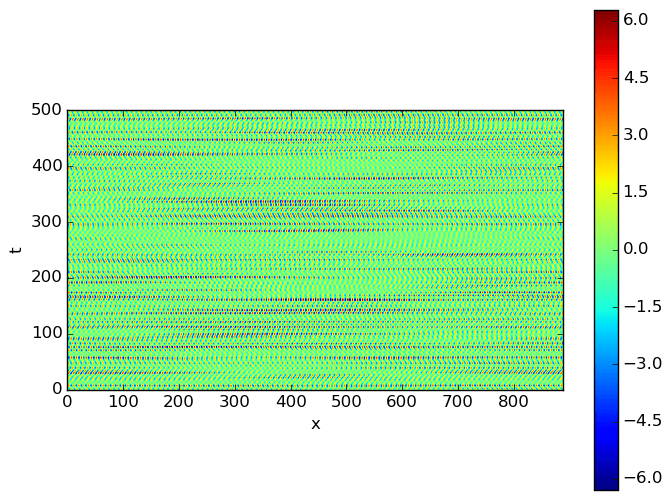
\includegraphics[width=\textwidth,height=.32\textheight]{MNG_T500L888_init}
\end{minipage}
\\
\begin{minipage}[height=.32\textheight]{.45\textwidth}
\centering \small{\texttt{(b)}}
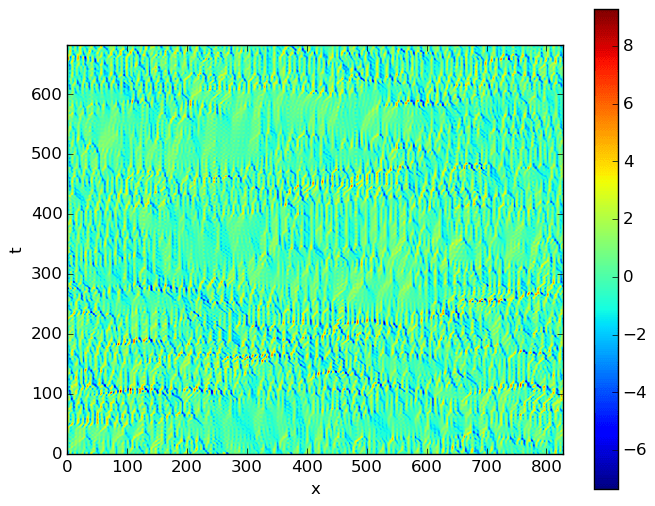
\includegraphics[width=\textwidth,height=.32\textheight]{MNG_T500L888_final}
\end{minipage}
\begin{minipage}[height=.32\textheight]{.45\textwidth}
\centering \small{\texttt{(c)}}
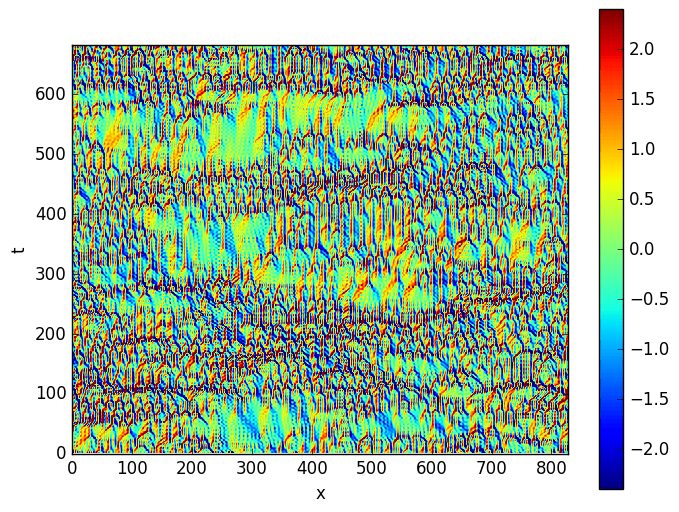
\includegraphics[width=\textwidth,height=.32\textheight]{MNG_T500L888_capped}
\end{minipage}
\caption{ \label{fig:MNG_spacetime_capped}
(a) Smoothed noise initialized on a spacetime domain $T=500$,
$L=100\,\bar{L} \approx 889$, where $\bar{L}=2\pi\sqrt{2}$.
Initial residual $F^2 = 16635$
(b) Resultant spatiotemporal field after one-hundred thousand adjoint descent
steps $F^2_f = 3.66$, $T_f = 682.62$, $L_f=828.31$.
(c) The same $u(x,t)$ as in (b), except with the displayed values constrained
between $-2.4 \leq u(x,t) \leq 2.4$. Computation time was approximately an hour
and ten minutes.
}
\end{figure}


\begin{figure}
\begin{minipage}[height=.05\textheight]{.3\textwidth}
\centering \small{\texttt{(a)}}\\
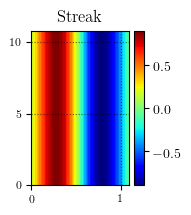
\includegraphics[width=.3\textwidth,height=.1\textheight]{MNG_streak}
\end{minipage}
\begin{minipage}[height=.05\textheight]{.3\textwidth}
\centering \small{\texttt{(b)}}\\
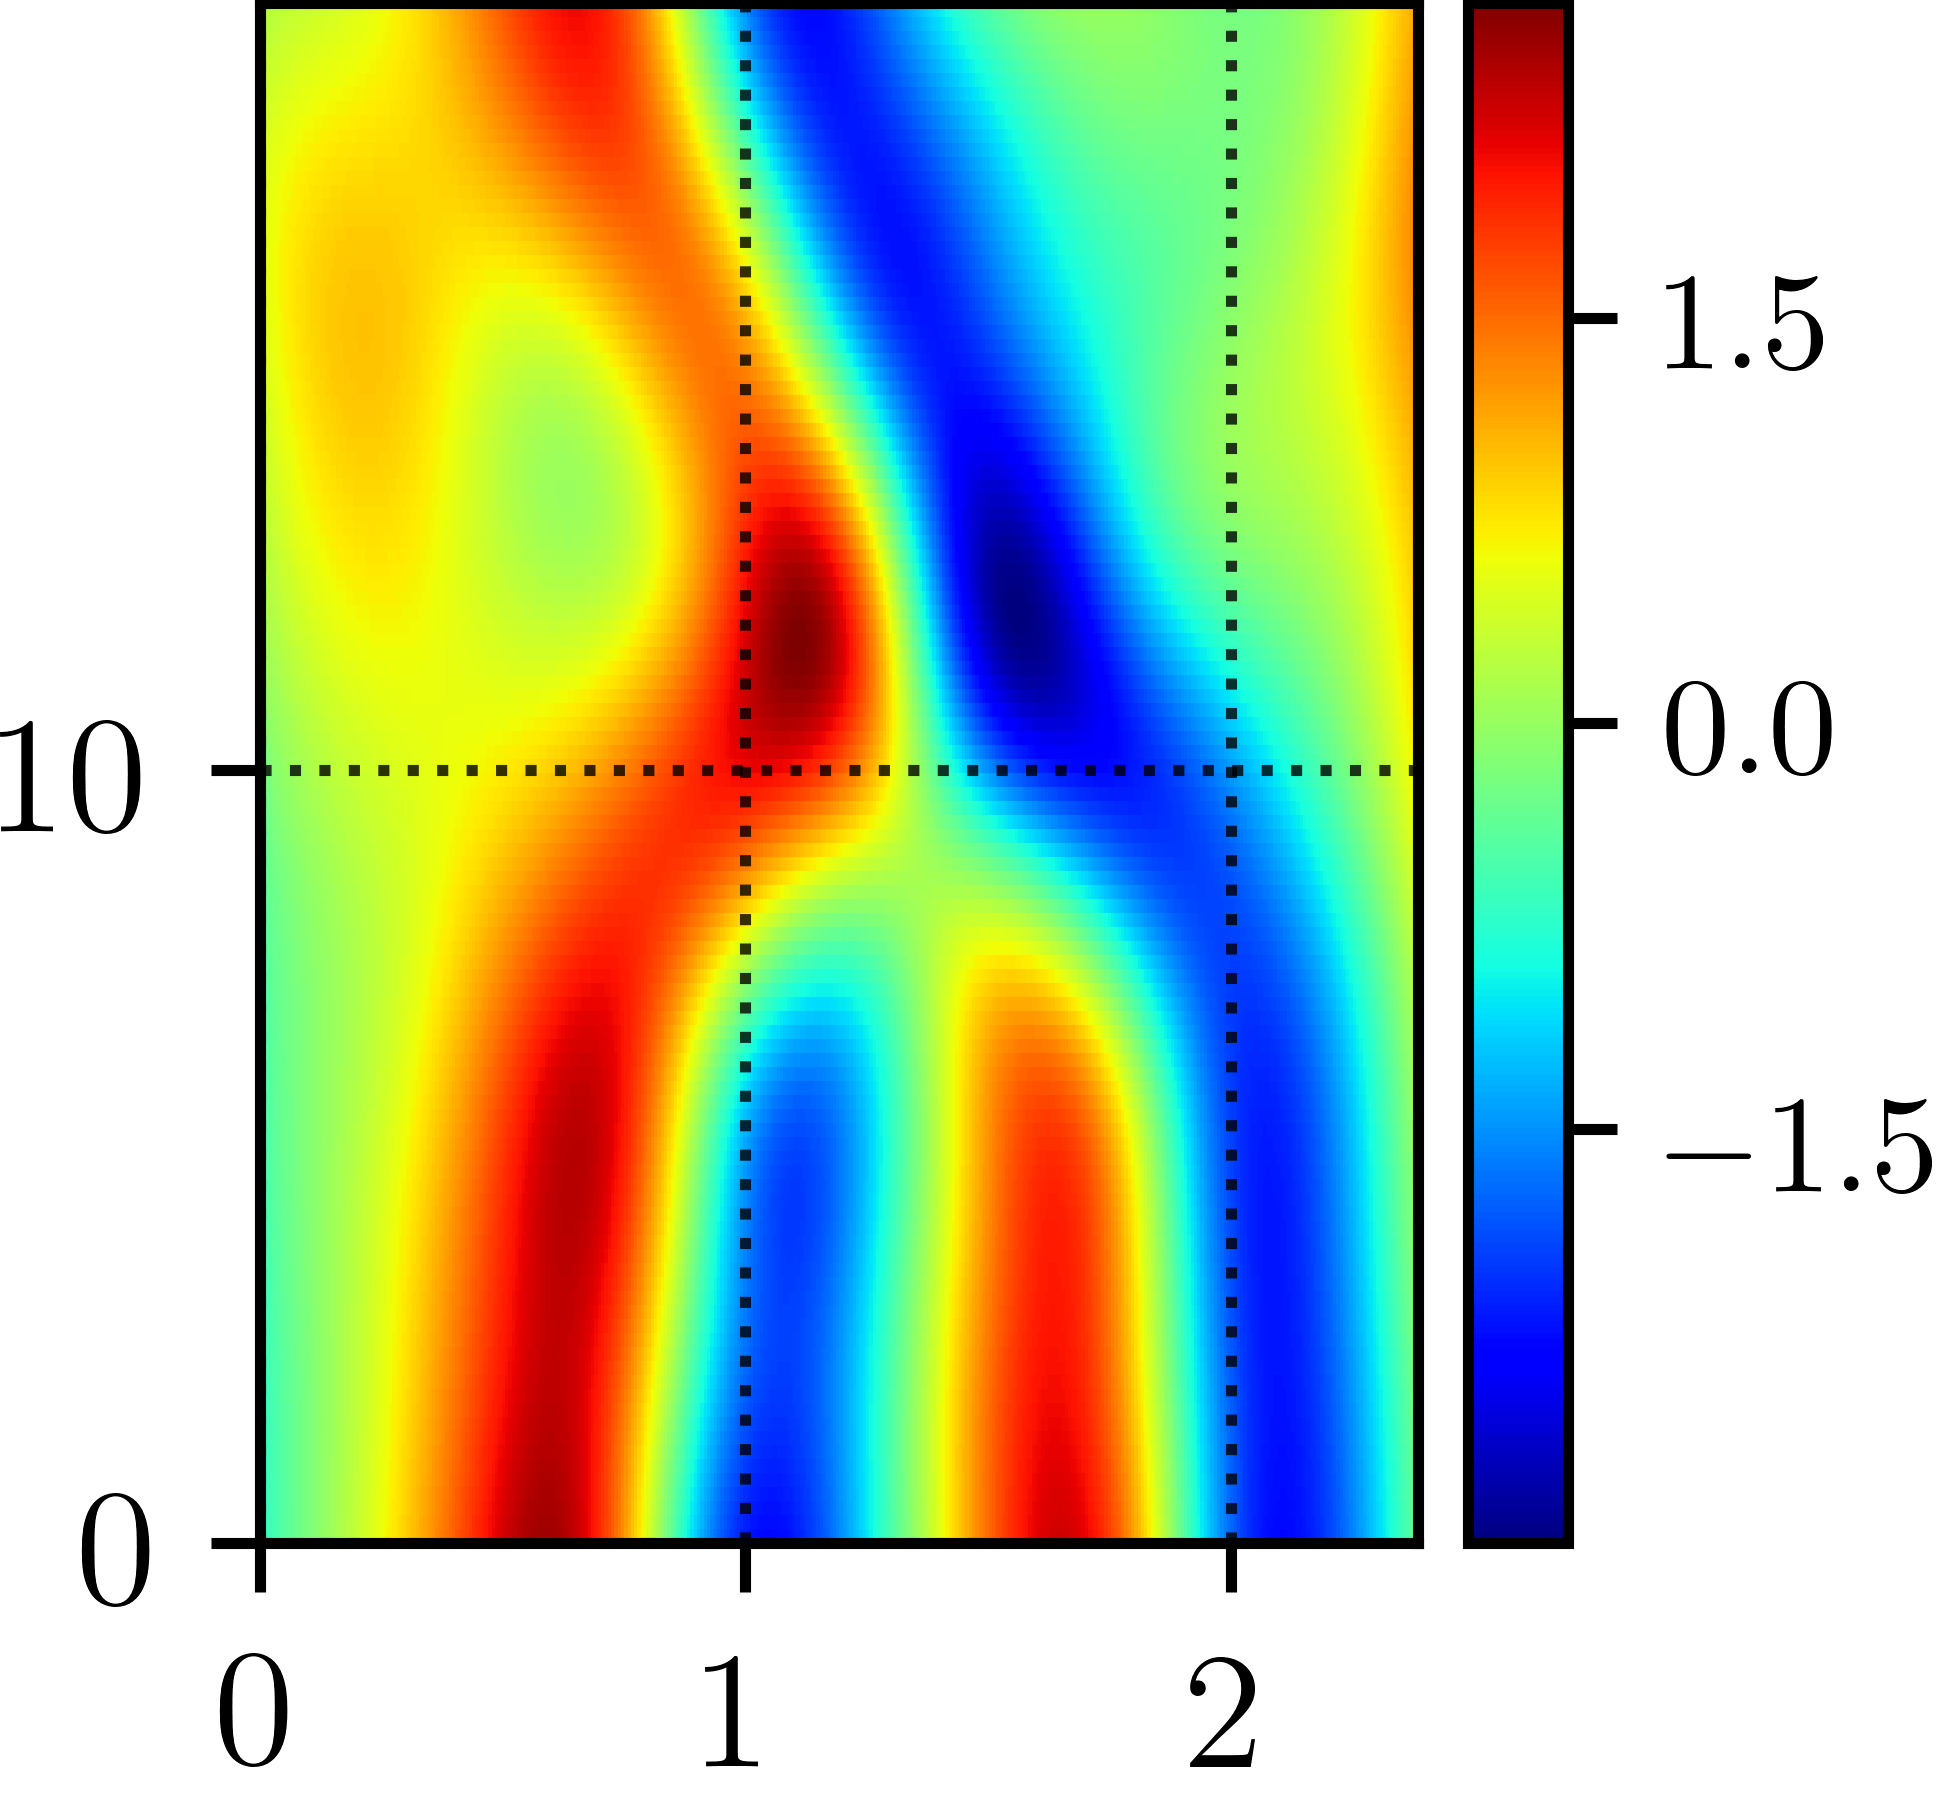
\includegraphics[width=.4\textwidth,height=.1\textheight]{MNG_hookondefecterg}
\end{minipage}
\begin{minipage}[height=.05\textheight]{.3\textwidth}
\centering \small{\texttt{(c)}}\\
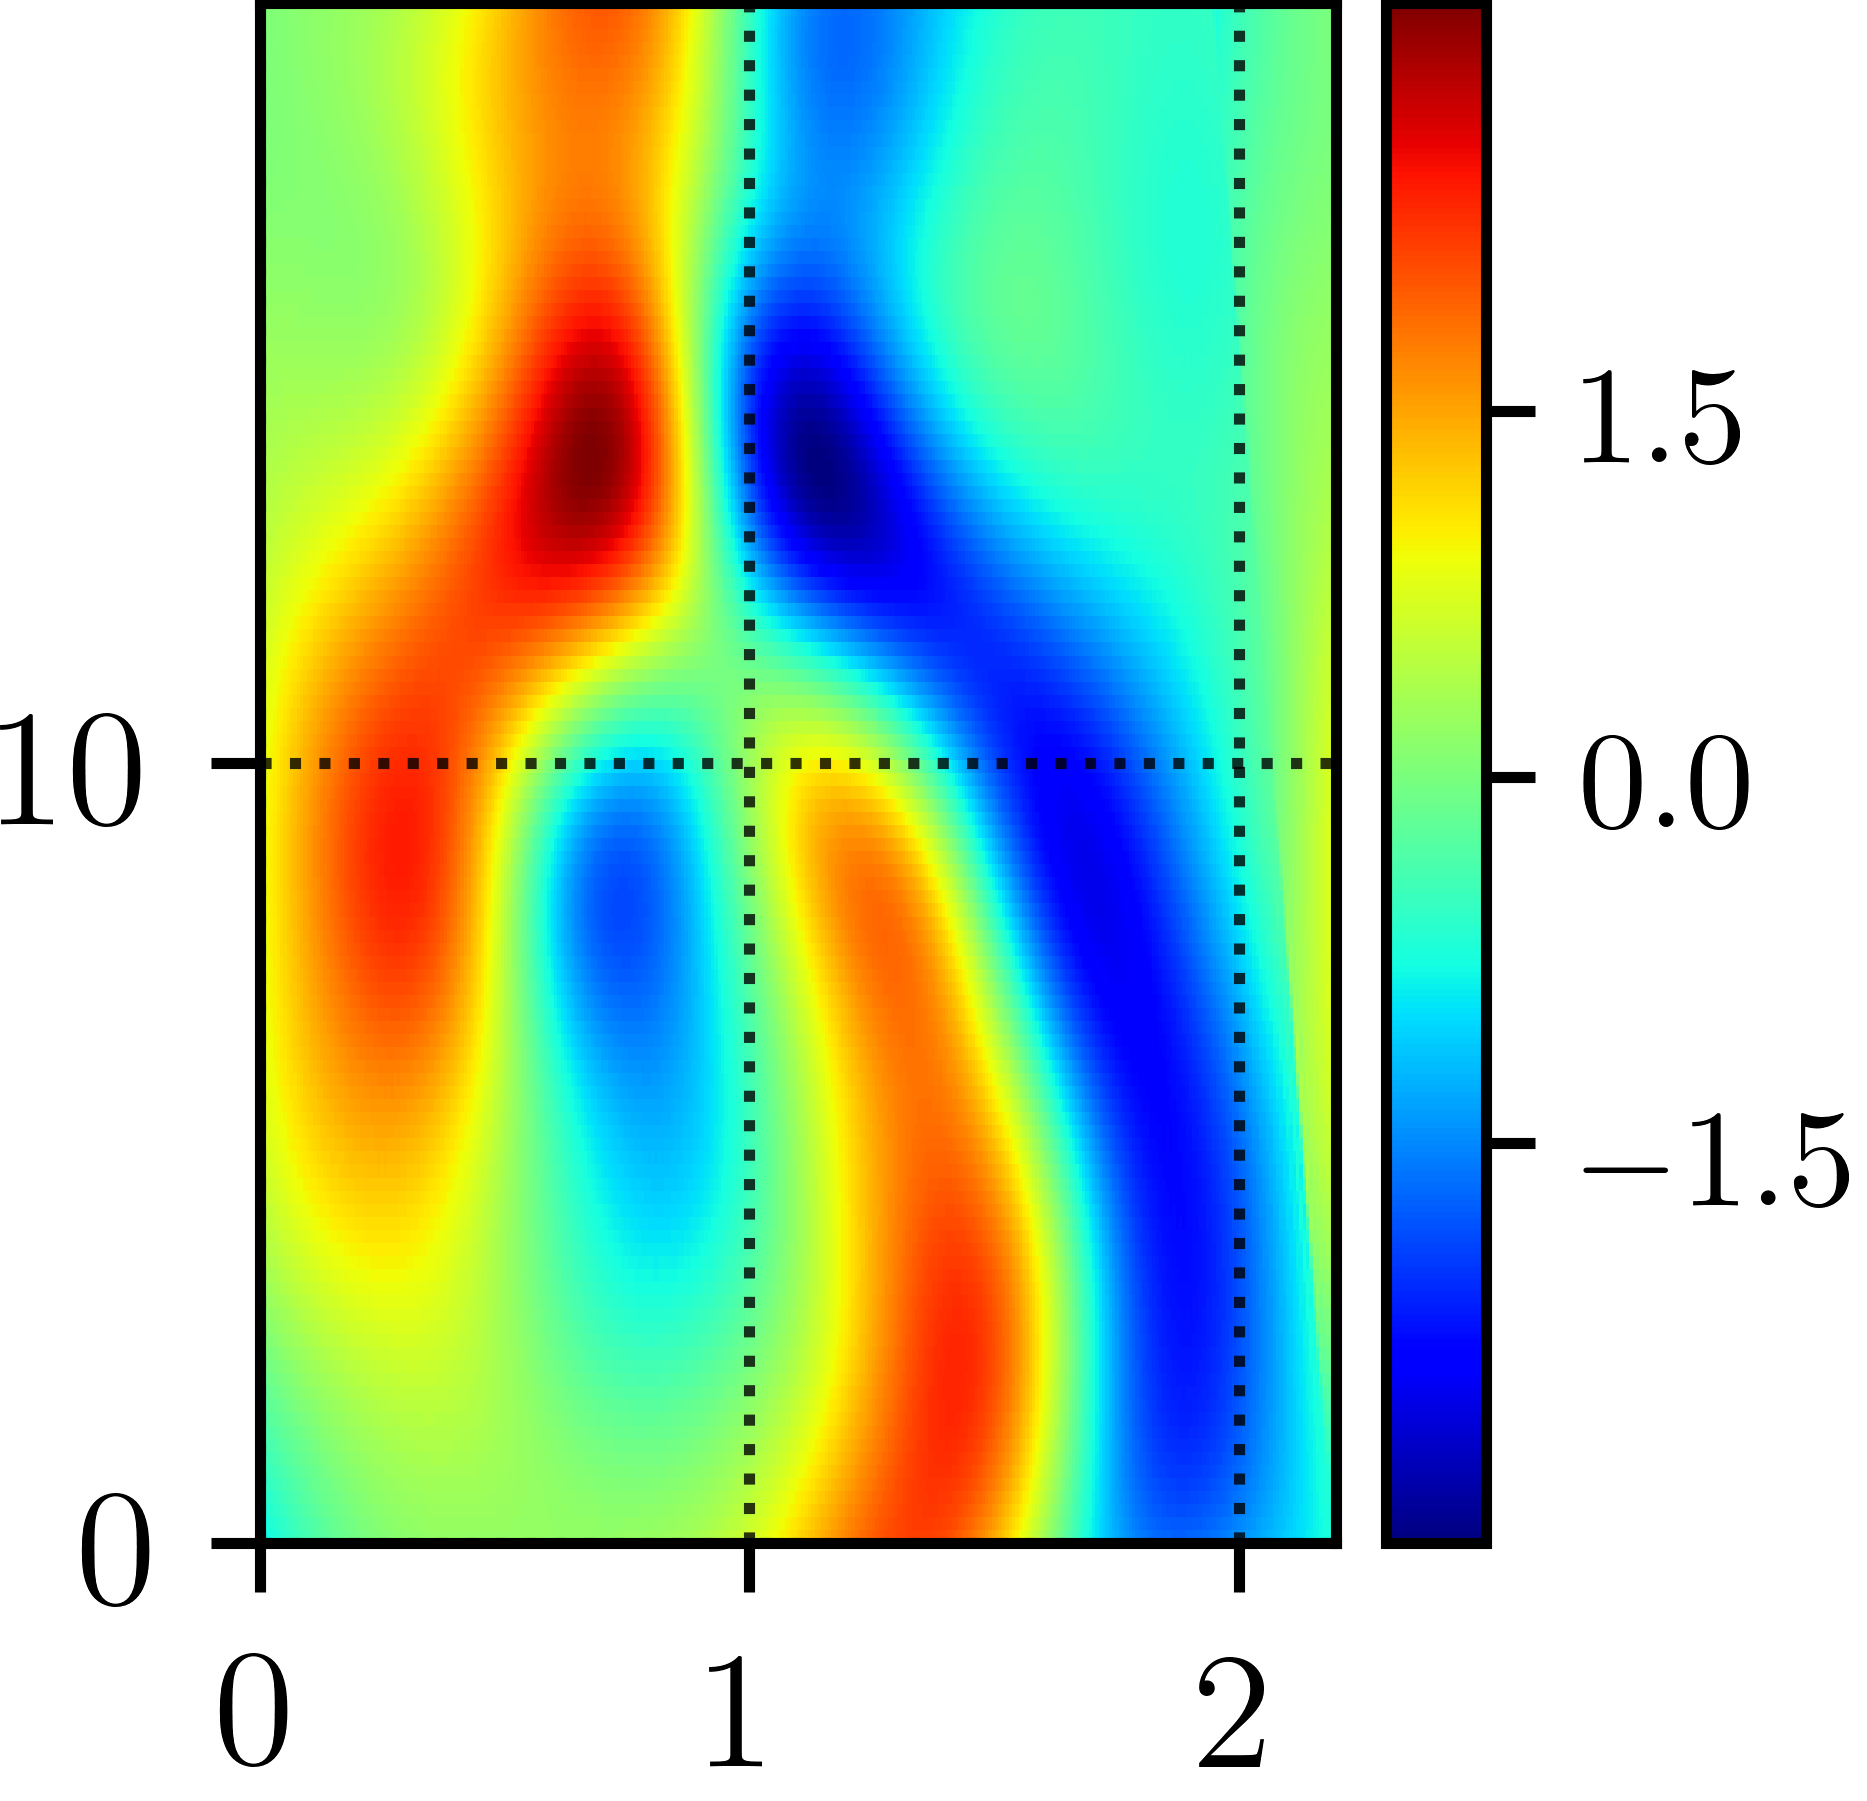
\includegraphics[width=.4\textwidth,height=.1\textheight]{MNG_halfdefecterg}
\end{minipage}
\begin{minipage}[height=.05\textheight]{.3\textwidth}
\centering \small{\texttt{(d)}}\\
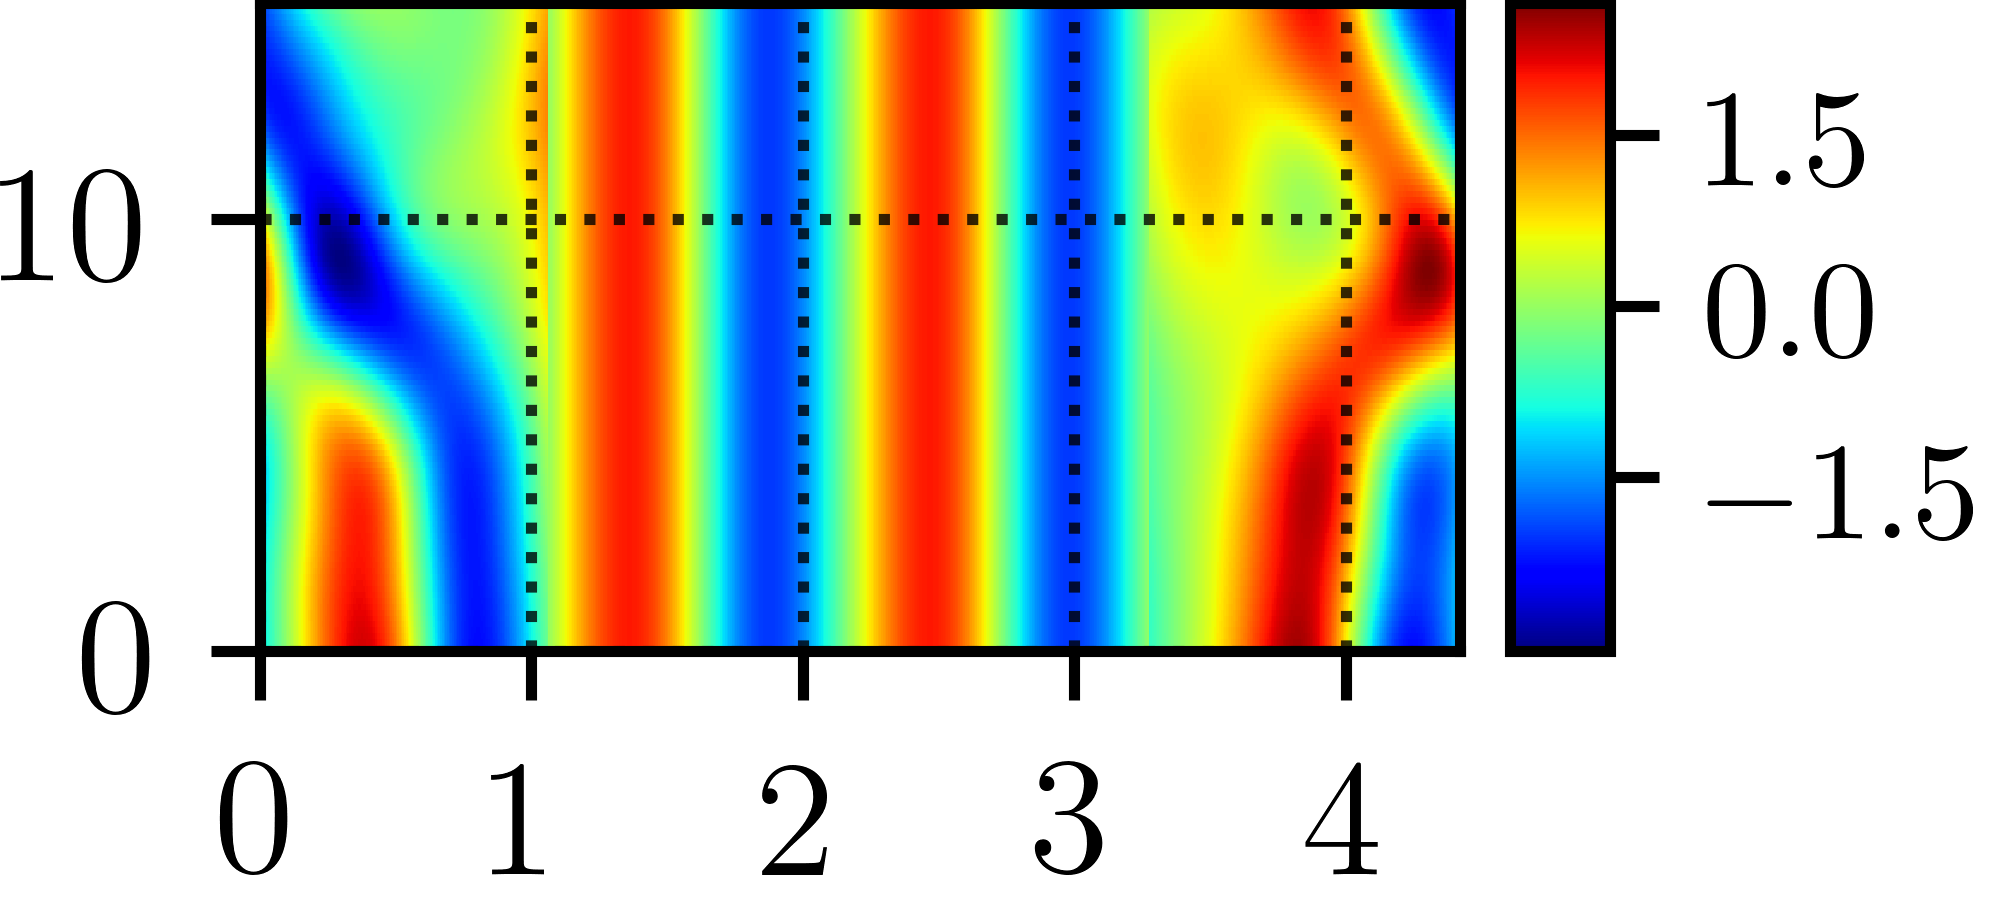
\includegraphics[width=.8\textwidth,height=.1\textheight]{MNG_tiling_subdomain0}
\end{minipage}
\begin{minipage}[height=.05\textheight]{.3\textwidth}
\centering \small{\texttt{(e)}}\\
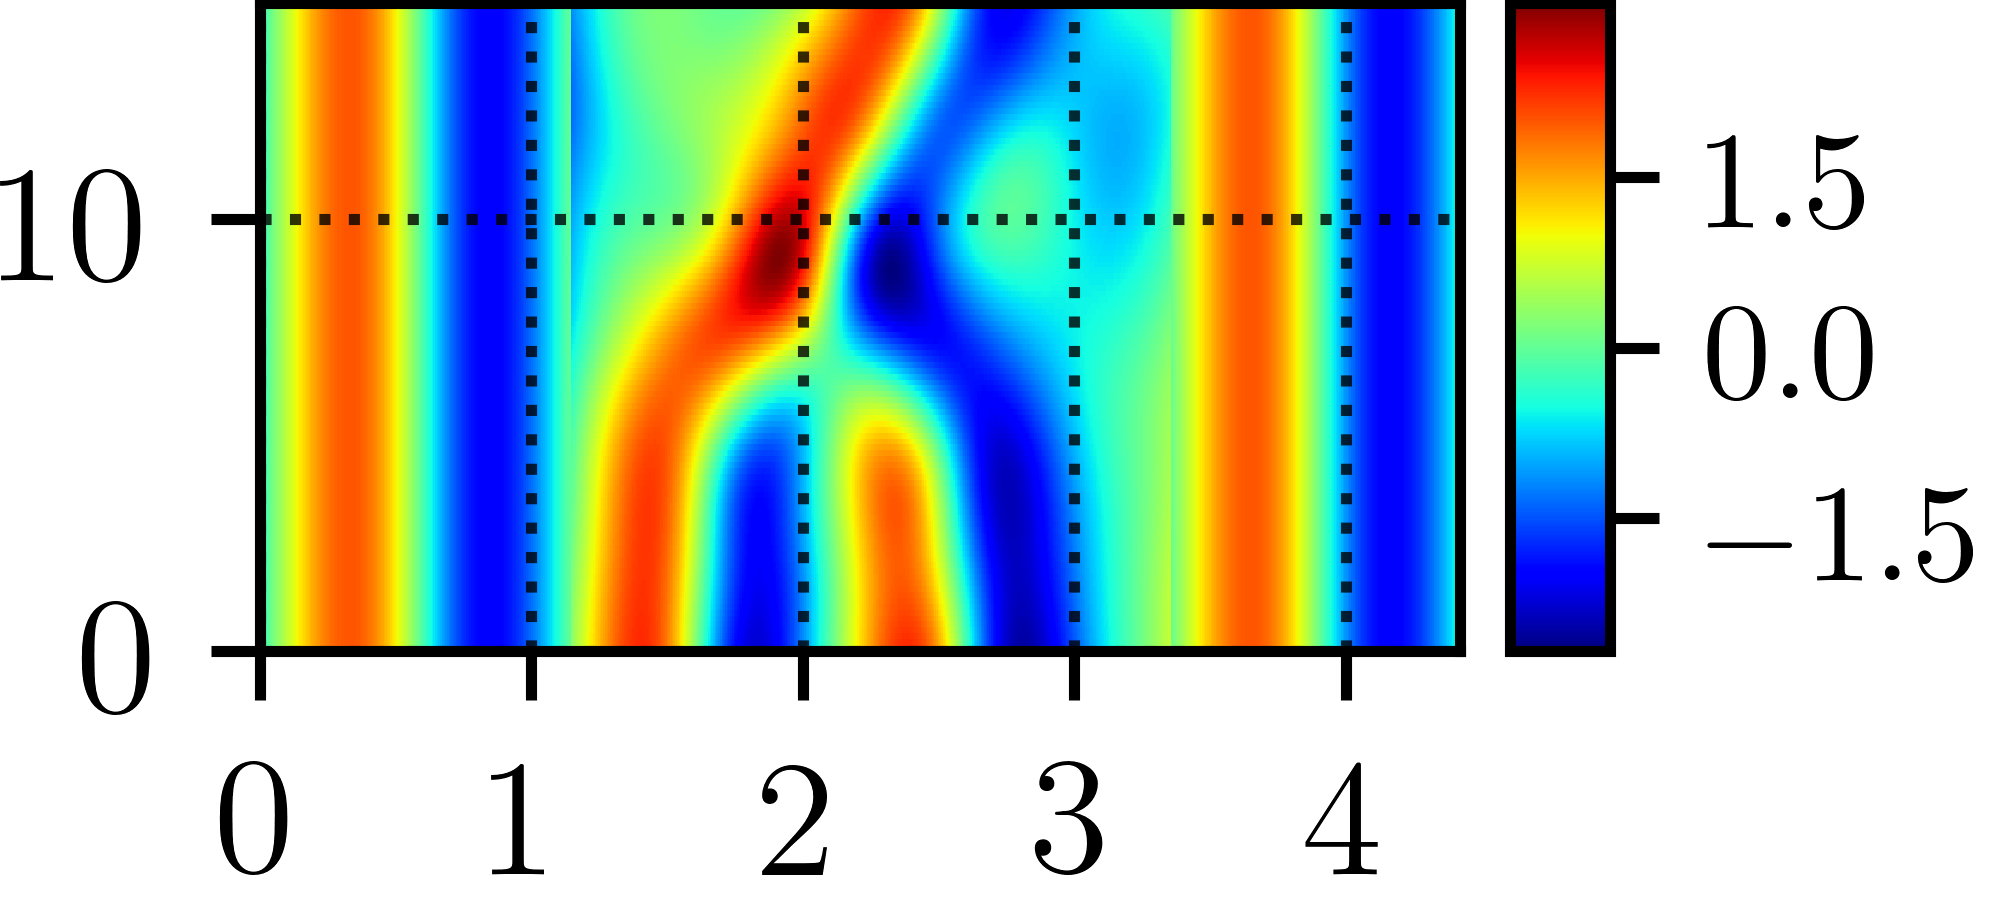
\includegraphics[width=.8\textwidth,height=.1\textheight]{MNG_tiling_subdomain1}
\end{minipage}
\begin{minipage}[height=.05\textheight]{.3\textwidth}
\centering \small{\texttt{(f)}}\\
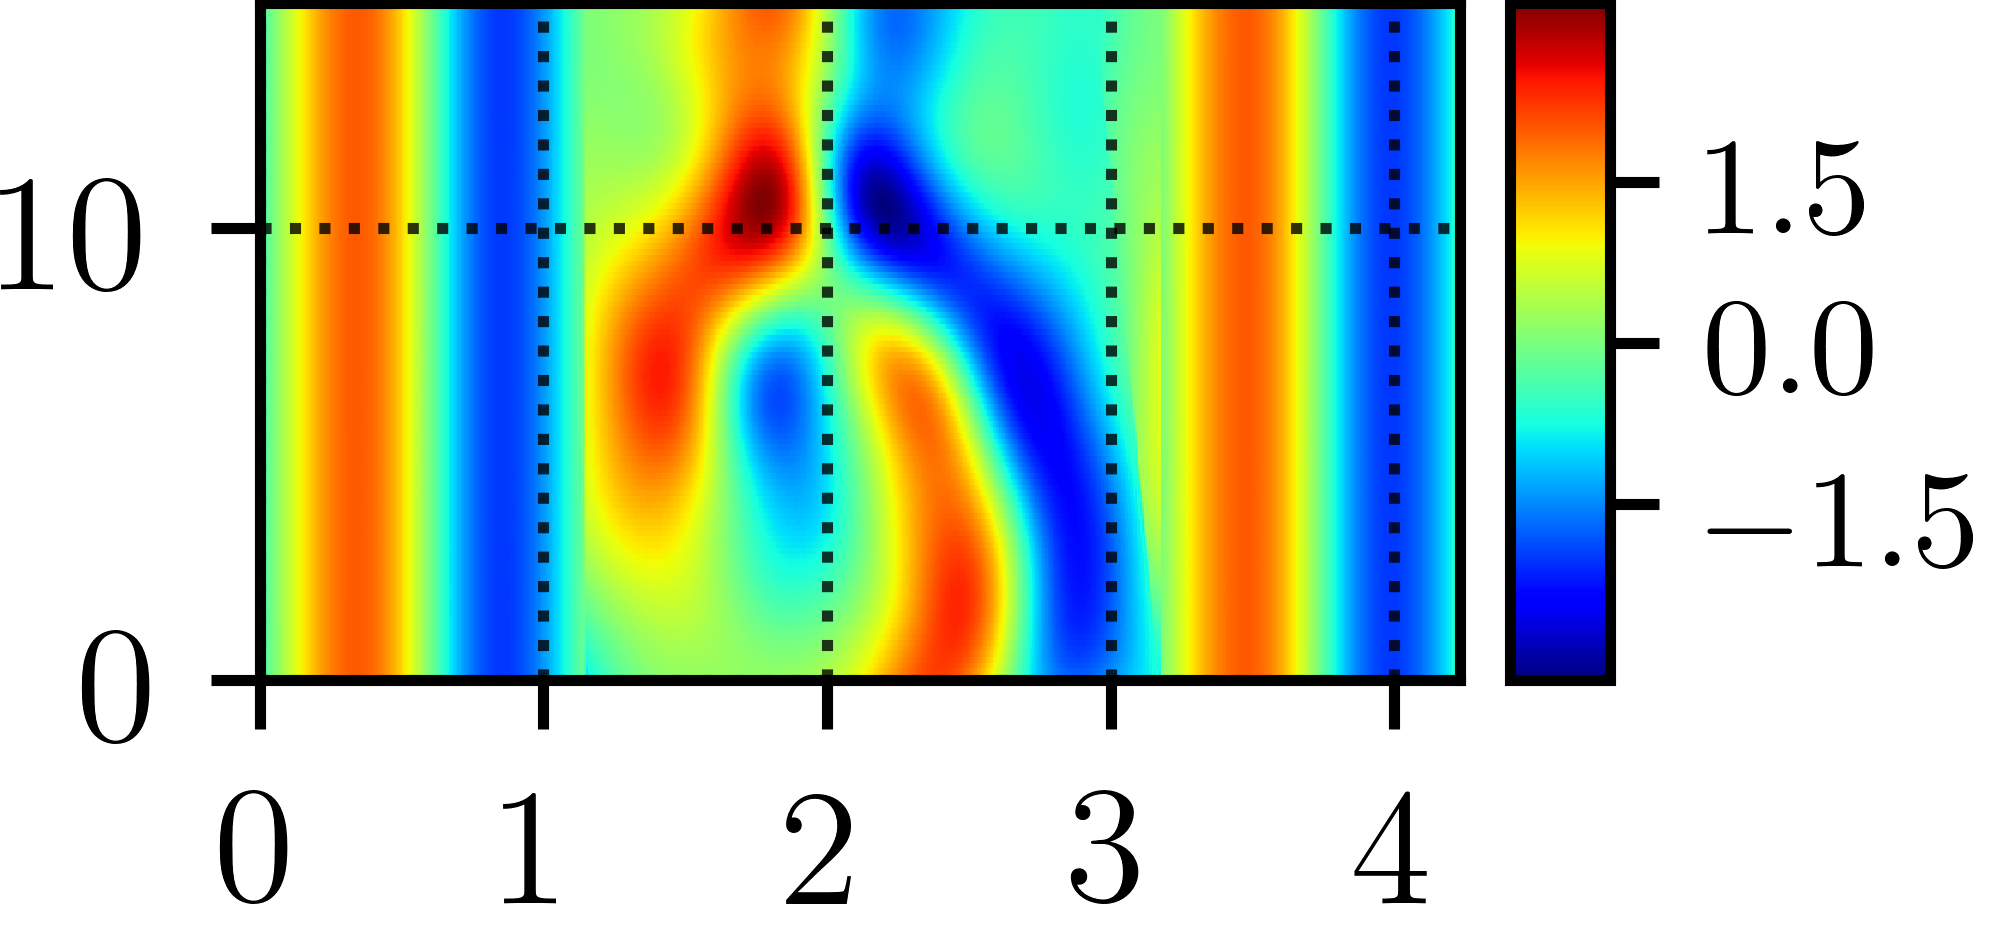
\includegraphics[width=.8\textwidth,height=.1\textheight]{MNG_tiling_subdomain2}
\end{minipage}
\begin{minipage}[height=.1\textheight]{.35\textwidth}
\centering \small{\texttt{(g)}}\\
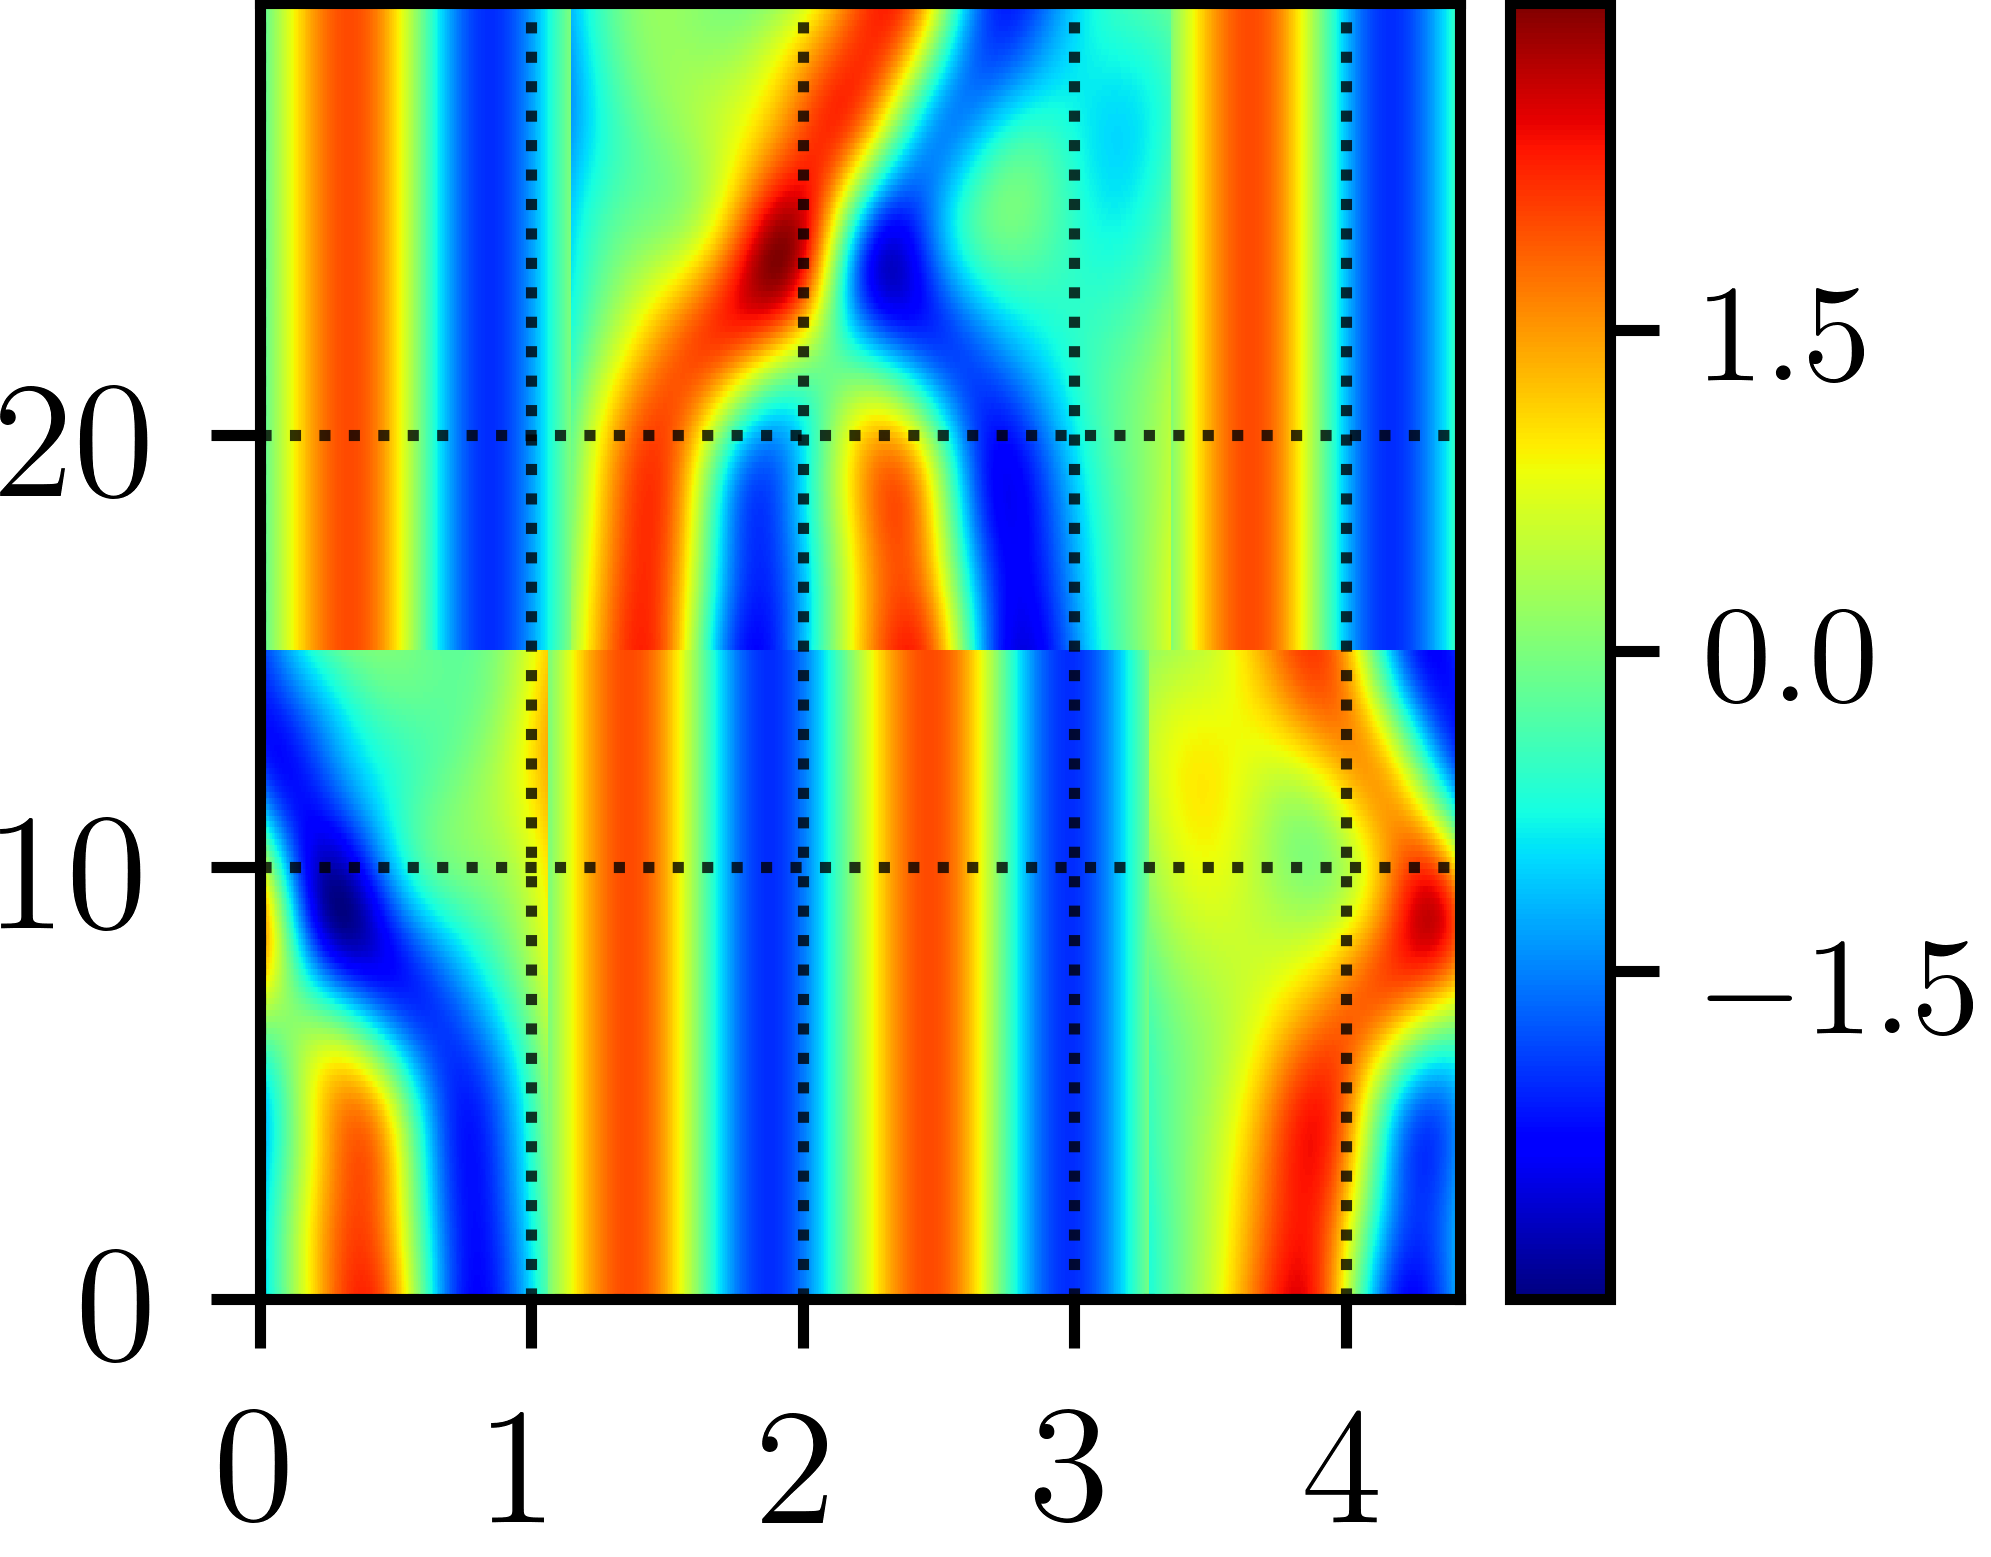
\includegraphics[width=.8\textwidth,height=.28\textheight]{MNG_tiling_twosubdomains}
\end{minipage}
\begin{minipage}[height=.15\textheight]{.3\textwidth}
\centering \small{\texttt{(h)}}\\
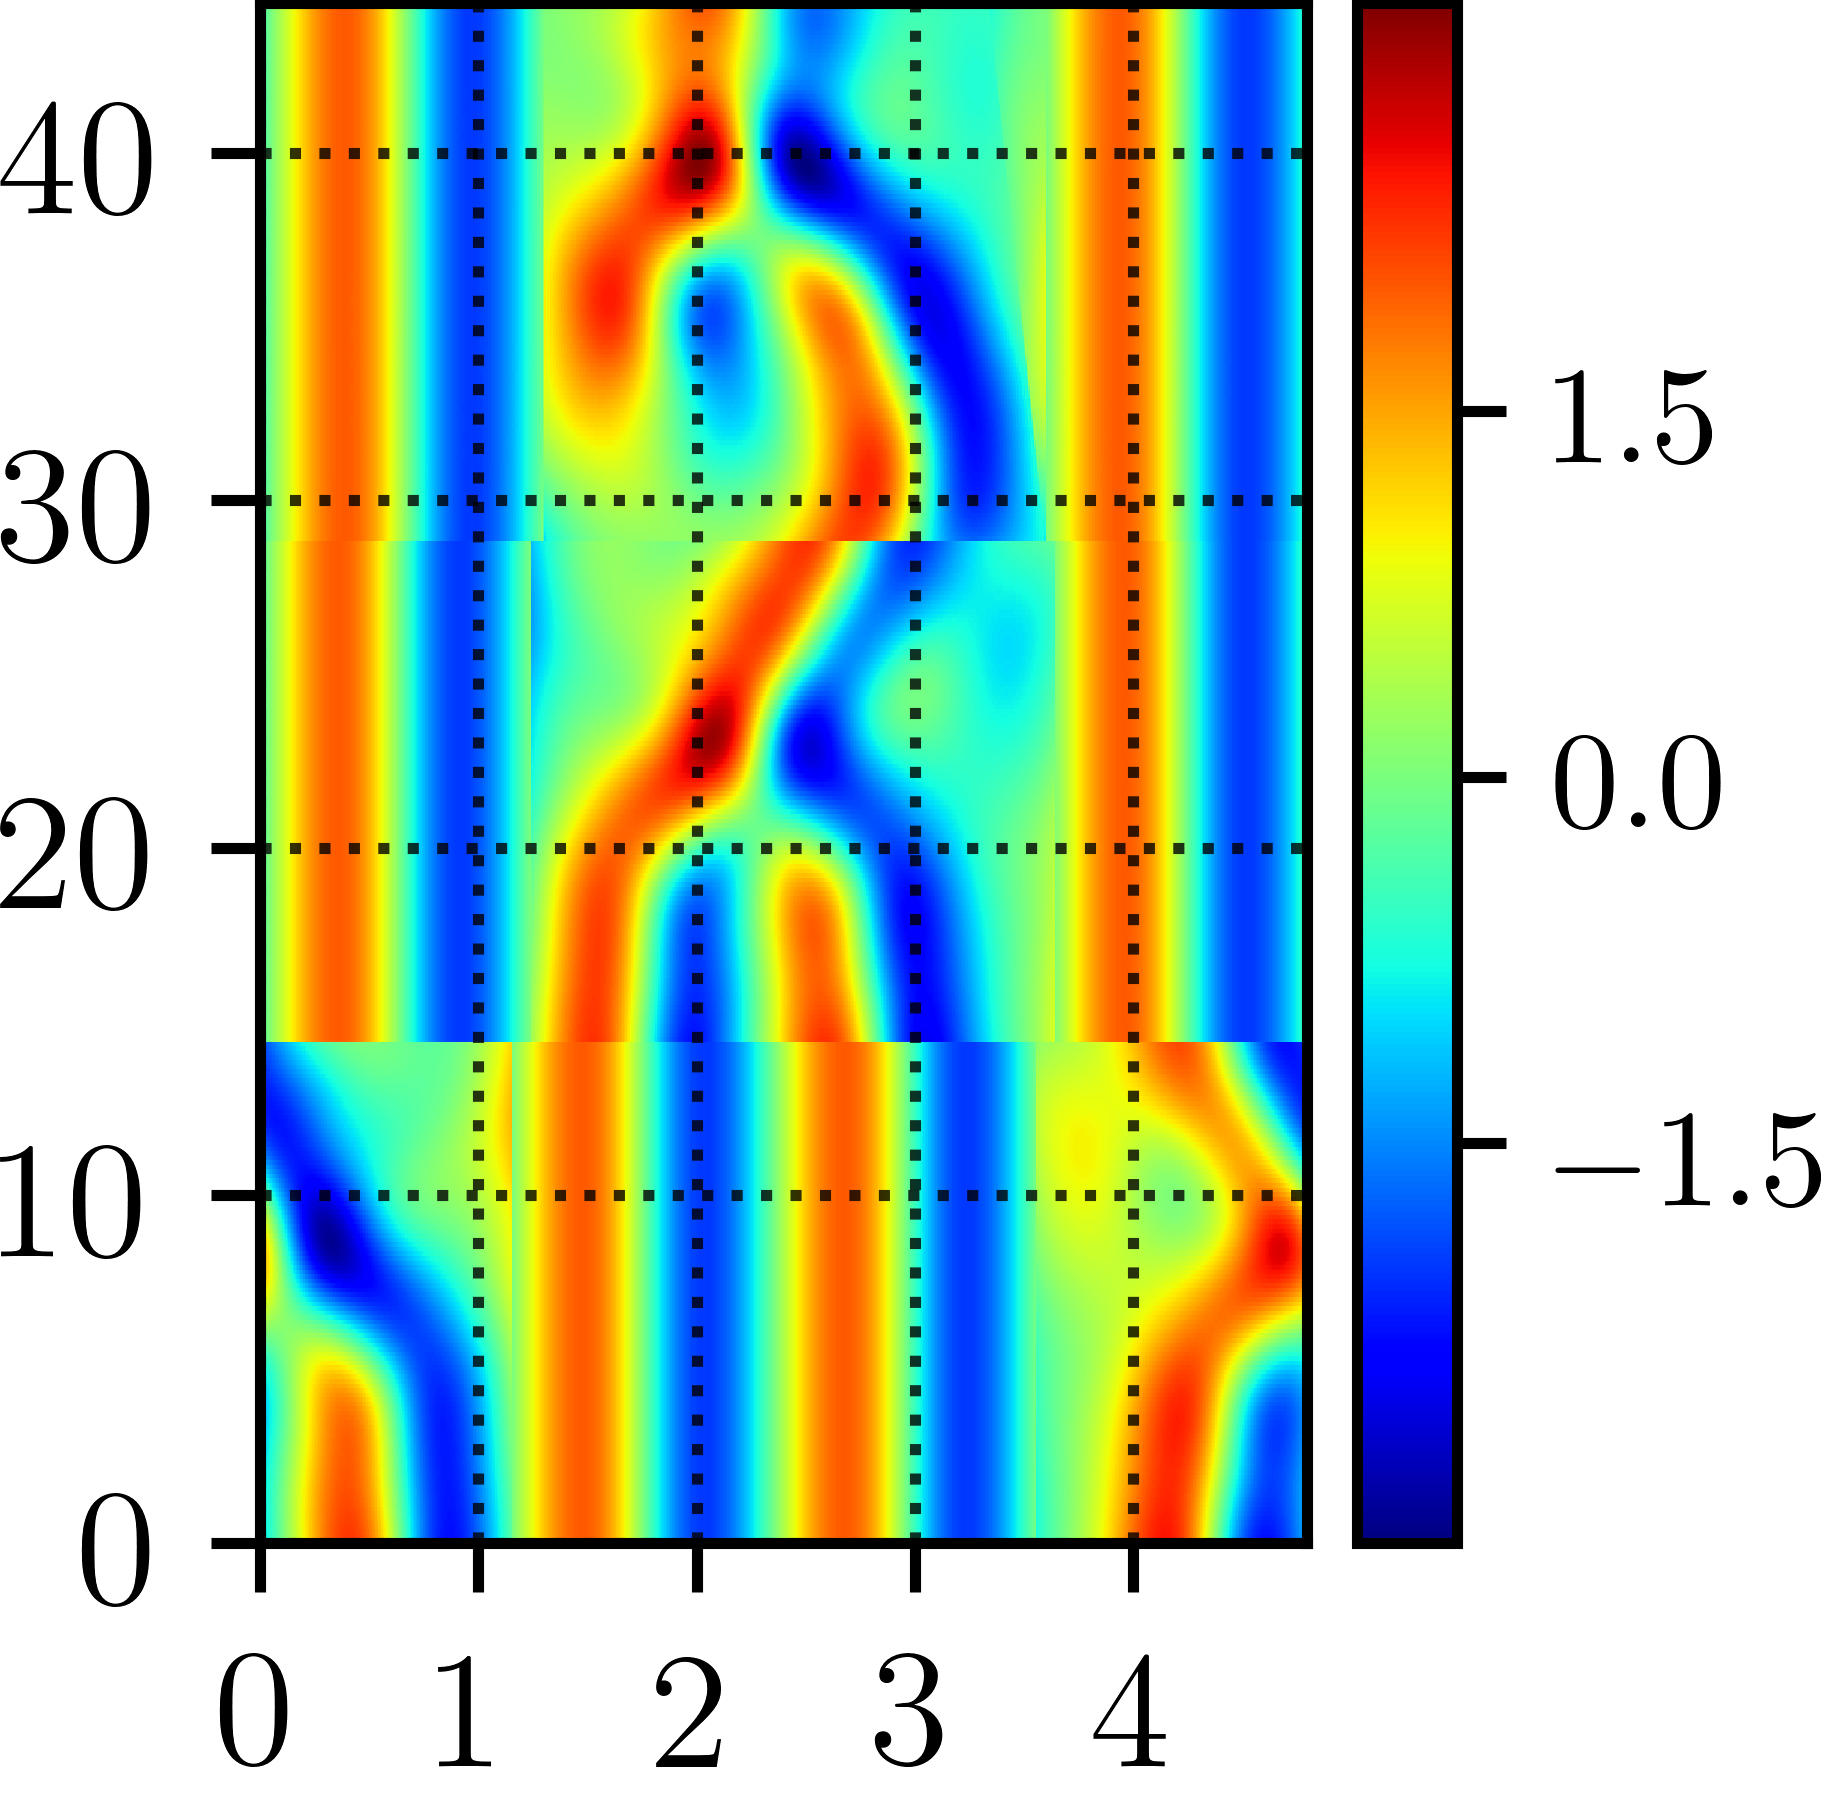
\includegraphics[width=\textwidth,height=.36\textheight]{MNG_tiling_fundamental}
\end{minipage}
\begin{minipage}[height=.15\textheight]{.3\textwidth}
\centering \small{\texttt{(i)}}\\
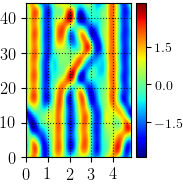
\includegraphics[width=\textwidth,height=.36\textheight]{MNG_tiling_initial}
\end{minipage}

\caption{ \label{fig:tilingschematic}
Demonstration of how to construct an initial condition corresponding to a specific
\spt\ symbolic block. (a),(b) and (c) together are the set of tiles used for all
other plots in this figure. (d) is a subdomain comprised of two copies of (a) and one copy of (b). (e) is a subdomain comprised of two copies of (a) and one copy of
the reflection of (b). (f) is a subdomain comprised of two copies of (a) and a
single copy of (c). The last row of figures demonstrate how to combine (d),(e),
and (f). (g) is the combination of (d) and (e). (h) is the combination of (d),(e)
and (f) (equivalently, (g) and (f)). Lastly (i) is the smoothed version of (h) which will serve as the initial condition.
}
\end{figure}

\begin{figure}
\begin{minipage}[height=.05\textheight]{\textwidth}
\centering
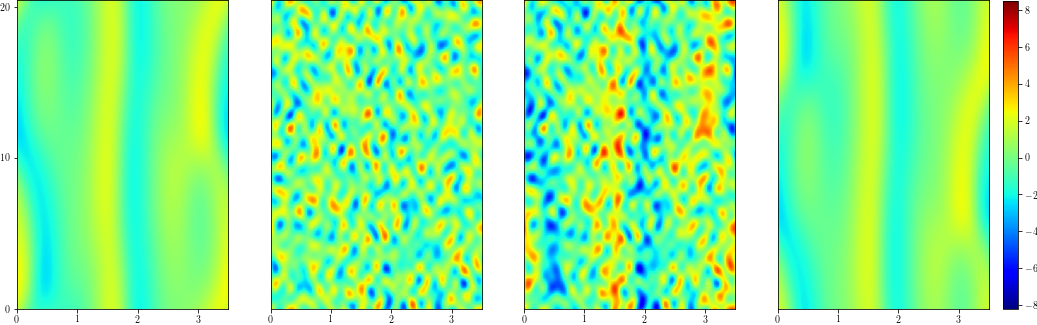
\includegraphics[width=1.0\textwidth,height=.2\textheight]{MNG_noise}
\end{minipage}
\caption{ \label{fig:MNGnoise}
(a) Original, converged \twot\ $[\speriod{}=21.99...,
\period{}=20.50...]$,
(b) aperiodic noise taken from standard normal distribution,
multiplied by
the $L_{\infty}$ norm of (a), (c) is the sum of (a) and (b),
(d) is the
\twot\ that (c) converges to, $[\speriod{}=22.18...,
\period{}=20.58...]$ .
}
\end{figure}

For a sense of how much noise is added, the maximum and
minimum values of
the fields in \reffig{fig:MNGnoise} are
(a) $\approx \pm 2.47$ and (c) $\approx \pm 8$. All four
fields are included
in a single figure to make it easier to have them share the
color legend. 